\documentclass[runningheads]{llncs}
%
\usepackage{graphicx}
\usepackage{booktabs}
\usepackage{soul}
\usepackage{color}
\usepackage{outlines}
\usepackage{amsmath}
\usepackage{amsfonts}
\usepackage{tikz}
\usetikzlibrary{positioning,arrows.meta} % for arrows
\usepackage{tabularx}
\newcolumntype{L}{>{\raggedright\arraybackslash}X}  % for Table 2 left justify
\usepackage{placeins} % for \FloatBarrier
% \usepackage{siunitx} 
\usepackage{lipsum}

%%% graphics, plots %%%
\usepackage{graphicx}
\usepackage{pgf, tikz}
\usepackage{pgfplots}
\pgfplotsset{compat=1.17}
\usepgfplotslibrary{statistics}
\usepackage{placeins}

\usepackage{subfig}
\usepackage[hidelinks]{hyperref}



% ALGOs
\usepackage{algorithm}% <======= http://ctan.org/pkg/algorithms
\usepackage{algpseudocode}% <=== http://ctan.org/pkg/algorithmicx
\algrenewcommand\algorithmicrequire{\textbf{Input:}}
\algrenewcommand\algorithmicensure{\textbf{Output:}}

% ALGO Numbering
% \renewcommand\thealgorithm{\thechapter.\arabic{algorithm}}  % e.g., 4.3 (Chap.Algo)
\renewcommand\thealgorithm{\thesection.\arabic{algorithm}} 		 % e.g., 4.1.3 (Chap.Sec.Algo)


% Used for Sci.Not.
\def\num#1{\numx#1}\def\numx#1e#2{{#1}\mathrm{e}{#2}}

% Orcid Line
\usepackage{orcidlink}

% Colors
\definecolor{sign}{HTML}{b02a2d}
\definecolor{direction}{HTML}{007900}
\definecolor{regime}{HTML}{8c399e}
\definecolor{characteristic}{HTML}{1f5dc2}
\definecolor{mantissa}{HTML}{636363}
\definecolor{error}{HTML}{BD002A}
\definecolor{cellbg}{HTML}{EDEDED}

\definecolor{posit}{HTML}{b02a2d}
\definecolor{bfloat16}{HTML}{007900}
\definecolor{float}{HTML}{636363}




\begin{document}
% High-Frequency 
\title{Depth or Breadth? Flat128 Arithmetic and the RV128 Opportunity}

%
\titlerunning{Flat128 Arithmetic and the RV128 Opportunity} 
%
% AUTHORS
% % -------------------------------
\author{Paul Sherman \inst{1}\orcidlink{0009-0000-3001-8285}  \and
Kurt Keville \inst{2}\orcidlink{0000-0003-0194-951X}}
%
\authorrunning{P. Sherman and K. Keville}%
%
\institute{RISC-V International; Posit Foundation
\and
Posit Foundation}
% 

% \author{First Author\inst{1}\orcidID{0000-1111-2222-3333} \and
% Second Author\inst{2,3}\orcidID{1111-2222-3333-4444} \and
% Third Author\inst{3}\orcidID{2222--3333-4444-5555}}
% %
% \authorrunning{F. Author et al.}
% % First names are abbreviated in the running head.
% % If there are more than two authors, 'et al.' is used.
% %
% \institute{Princeton University, Princeton NJ 08544, USA \and
% Springer Heidelberg, Tiergartenstr. 17, 69121 Heidelberg, Germany
% \email{lncs@springer.com}\\
% \url{http://www.springer.com/gp/computer-science/lncs} \and
% ABC Institute, Rupert-Karls-University Heidelberg, Heidelberg, Germany\\
% \email{\{abc,lncs\}@uni-heidelberg.de}}


 


% AFFILIATIONS
% -------------------------------
 
% -------------------------------

  
 
% -------------------------------



% AFFILIATIONS
% -------------------------------
%\institute{University of Southern Maine, ME 04104, USA \\
%\email{name@college.edu}}
% Multiple authors/institutions
% \institute{Another Place\\
% \email{author@company.com} \\
% \url{https://company.com} \and
% Some plance \\
%\email{name@college.edu}}
% 
% -------------------------------



\maketitle % Makes title, authors, etc. 

\begin{abstract}
IEEE 754 floating-point arithmetic partitions each register into exponent
and mantissa, purchasing dynamic range at the cost of precision,
reproducibility, and semantic transparency. We argue this tradeoff is
increasingly unfavorable for modern workloads such as neural network
inference, scientific accumulation, and auditable high-precision
reductions, where the exponent field spends bits on range that is never
needed. The sigmoid activation function, central to modern neural
networks, saturates outside the interval roughly $[-6, 6]$ --- a range
requiring fewer than four bits of integer part --- yet IEEE~754's
float32 spends 8 exponent bits purchasing range to $\pm3.4\times10^{38}$
for this computation. FP8 formats have begun to address this mismatch at
inference time; posit8 with es=1 addresses it more elegantly through
tapered precision. We address the complementary problem at the
accumulator layer, where gradient magnitudes during training can span ten
or more orders of magnitude yet must be summed with sufficient precision
to distinguish meaningful updates from numerical noise.

We propose flat128, an optional wide fixed-point extension for RISC-V
that treats a 128-bit register as a uniform two's complement significand
with compiler-managed binary point. No bits are sacrificed to exponent
overhead. Addition and subtraction are exact when operands share a scale.
Multiplication yields a 256-bit exact intermediate product; narrowing is
explicit and architecturally specified, never hidden. Accumulation is
bitwise reproducible across conforming implementations without
per-operation rounding --- a contract IEEE~754 cannot offer without
simultaneously fixing format, rounding mode, operation sequence, and
contraction behavior. We demonstrate this experimentally: flat128
accumulation of dot products from 64 to 4096 elements yields
bitwise-identical results across 1 and 64 concurrent threads on all four
NUMA nodes of the SG2042 (64-hart RISC-V); IEEE~754 double-precision
accumulation of identical inputs diverges by up to $8.9\times10^{-16}$
at $K=4096$.

\keywords{
  SV/128 \and
  flat128 \and
  RISC-V \and
  reproducibility \and
  fixed-point arithmetic \and 
  posits \and 
  wide accumulation
}

\textbf{AMS subject classifications}: {65N55, 65F10}
\end{abstract}


% user definitions
\def\fp#1{\texttt{Float#1}}
\def\bf{\texttt{BFloat16}}
\def\p#1{\texttt{Posit#1}}

% ---- Section: Intro. ----
\section{Introduction}\label{sec:intro}
IEEE 754 floating-point arithmetic partitions each register into exponent
and mantissa, purchasing dynamic range at the cost of precision,
reproducibility, and semantic transparency. This tradeoff is increasingly
unfavorable for modern workloads, especially neural network inference
and scientific accumulation, where the exponent field spends bits on
range that is neither needed nor used.

We propose flat128, an optional wide fixed-point extension for RISC-V,
useful on RV64, RV128, and vector-capable machines, that makes
accumulation width, scale, narrowing, and overflow architecturally
explicit. RV128's 128-bit integer registers are a convenient scalar
substrate; the argument does not depend on them.

The proposal is complementary to Gustafson's posit arithmetic rather
than competitive with it. Posits address where precision bits go within
a narrow operand; flat128 addresses where result bits go across a wide
accumulation. Both are attacks on the same root cause: IEEE~754 hides
rounding from the programmer and accumulates error invisibly~\cite{ieee2019standard}. The natural
division of labor is posit8/16 at the activation layer and flat128 at
the accumulator layer~\cite{gustafson2017beating,gustafson2017end}.

Flat128 differs from conventional fixed-point arithmetic in two respects. First, the binary point is compiler-managed rather than programmer-managed, eliminating the manual scaling discipline that makes fixed-point error-prone in practice. Second, flat128 accumulation is bitwise reproducible across arbitrary thread counts and NUMA domains---a property naive fixed-point does not provide and IEEE~754 explicitly sacrifices for performance. The reproducibility guarantee follows directly from the absence of exponent fields: with a shared binary point, partial sums commute exactly and thread-order dependence vanishes. We demonstrate this empirically on a 64-hart RISC-V platform.

The extension is designed for minimum deployment friction. It requires no
new number format in the compiler, since GCC and LLVM already support
\texttt{\_\_uint128\discretionary{}{}{\_}t}. It introduces no new rounding modes. It does not break existing ABI\@. A working partial-product multiply demonstration in portable C, \texttt{Mult128.c} ~\cite{sherman2026mult128},
shows that a $128\times128$-bit product reduces to sixteen $32\times32$
partial products, each mapping to a single RV64I MUL instruction, with
no exotic hardware required. The ISA encoding sketch fits within the
existing 32-bit instruction word using six standard RISC-V instruction
forms R(4), I, S, B, U, and J\@.

Open architectural questions such as binary point convention, register
file design, overflow semantics, and memory ABI are identified explicitly
and treated as a research agenda rather than resolved claims. The
publishable thesis is this: make accumulation width, scale, narrowing,
and overflow architecturally explicit, then measure whether that beats
existing FMA and vector approaches for defined workloads. That question
is technically serious. We intend to answer it.

\subsection{The Segment Register Analogy}

x86 real-mode segmentation added artificial addressing range through
SS/DS/ES register indirection at the cost of programmer complexity,
hardware pain, and decades of legacy burden. IEEE~754 commits the same
sin arithmetically: exponent bits simulate range that could instead fund
precision.

\begin{figure}[h]
\centering
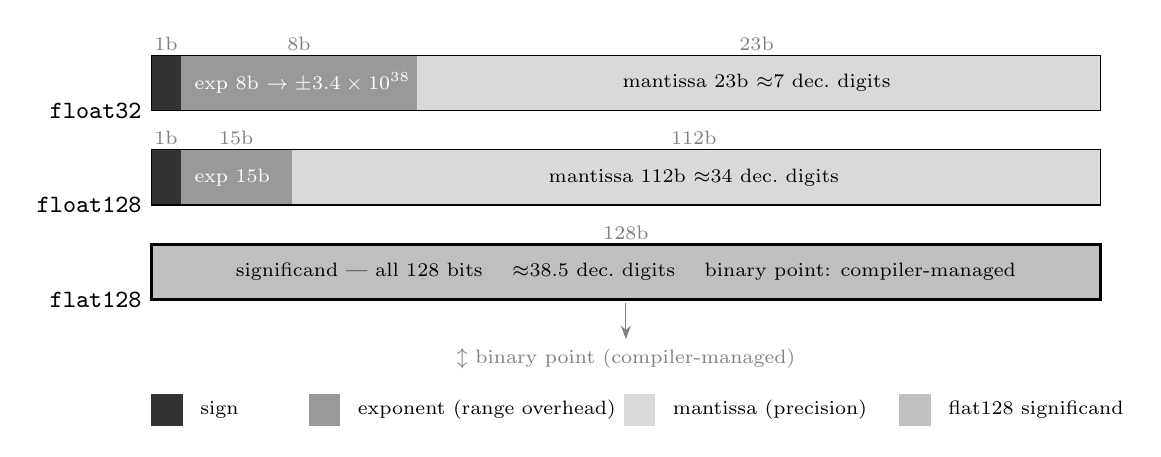
\begin{tikzpicture}[font=\small]
  \def\W{\dimexpr\textwidth-2pt\relax}
  \def\H{0.7}
  \def\gap{1.2}
  \def\fsign{0.375}
  \def\fexp{3.0}
  \def\fmant{8.625}
  \node[anchor=east] at (0, 0)       {\texttt{float32}};
  \node[anchor=east] at (0, -\gap)   {\texttt{float128}};
  \node[anchor=east] at (0, -2*\gap) {\texttt{flat128}};
  \fill[black!80] (0,0) rectangle (\fsign,\H);
  \fill[black!40] (\fsign,0) rectangle (\fsign+\fexp,\H);
  \fill[black!15] (\fsign+\fexp,0) rectangle (\W,\H);
  \draw (0,0) rectangle (\W,\H);
  \node[white,anchor=west,font=\scriptsize] at (\fsign+0.05, \H/2) {exp 8b $\rightarrow\pm3.4\times10^{38}$};
  \node[anchor=center,font=\scriptsize] at (\fsign+\fexp+\fmant/2, \H/2) {mantissa 23b $\approx$7 dec.\ digits};
  \node[font=\scriptsize,gray] at (\fsign/2,       \H+0.15) {1b};
  \node[font=\scriptsize,gray] at (\fsign+\fexp/2, \H+0.15) {8b};
  \node[font=\scriptsize,gray] at (\fsign+\fexp+\fmant/2, \H+0.15) {23b};
  \def\fhsign{0.375}
  \def\fhexp{1.406}
  \def\fhmant{10.219}
  \fill[black!80] (0,-\gap) rectangle (\fhsign,-\gap+\H);
  \fill[black!40] (\fhsign,-\gap) rectangle (\fhsign+\fhexp,-\gap+\H);
  \fill[black!15] (\fhsign+\fhexp,-\gap) rectangle (\W,-\gap+\H);
  \draw (0,-\gap) rectangle (\W,-\gap+\H);
  \node[white,anchor=west,font=\scriptsize] at (\fhsign+0.05,-\gap+\H/2) {exp 15b};
  \node[anchor=center,font=\scriptsize] at (\fhsign+\fhexp+\fhmant/2,-\gap+\H/2)
        {mantissa 112b $\approx$34 dec.\ digits};
  \node[font=\scriptsize,gray] at (\fhsign/2,      -\gap+\H+0.15) {1b};
  \node[font=\scriptsize,gray] at (\fhsign+\fhexp/2,-\gap+\H+0.15) {15b};
  \node[font=\scriptsize,gray] at (\fhsign+\fhexp+\fhmant/2,-\gap+\H+0.15) {112b};
  \fill[black!25] (0,-2*\gap) rectangle (\W,-2*\gap+\H);
  \draw[very thick] (0,-2*\gap) rectangle (\W,-2*\gap+\H);
  \node[anchor=center,font=\scriptsize,black] at (\W/2,-2*\gap+\H/2)
        {significand --- all 128 bits \quad $\approx$38.5 dec.\ digits
         \quad binary point: compiler-managed};
  \node[font=\scriptsize,gray] at (\W/2,-2*\gap+\H+0.15) {128b};
  \draw[-{Stealth},gray] (\W/2,-2*\gap-0.05) -- (\W/2,-2*\gap-0.5)
        node[below,font=\scriptsize,gray] {$\updownarrow$ binary point (compiler-managed)};
  \fill[black!80] (0,-4.0) rectangle (0.4,-3.6); \node[anchor=west,font=\scriptsize] at (0.5,-3.8) {sign};
  \fill[black!40] (2,-4.0) rectangle (2.4,-3.6); \node[anchor=west,font=\scriptsize] at (2.5,-3.8) {exponent (range overhead)};
  \fill[black!15] (6,-4.0) rectangle (6.4,-3.6); \node[anchor=west,font=\scriptsize] at (6.5,-3.8) {mantissa (precision)};
  \fill[black!25] (9.5,-4.0) rectangle (9.9,-3.6); \node[anchor=west,font=\scriptsize] at (10,-3.8) {flat128 significand};
\end{tikzpicture}
\caption{Bit allocation in float32, float128, and flat128. The exponent
field purchases dynamic range at the cost of significand bits. Flat128
eliminates the exponent entirely; the binary point is compiler-managed
metadata, not architectural state.}
\label{fig:bitalloc}
\end{figure}

\subsection{Context: Gustafson and Posit Arithmetic}

Gustafson's unum/posit work delivers tapered precision with maximum
significand bits near $\pm1.0$. Posit8 with es=1 matches the tapered
precision to sigmoid, softmax, and weight distributions; accuracy against FP8/BF16 baselines must be measured. The quire provides exact
dot product accumulation without intermediate rounding~\cite{posits-standard-2022}. The key insight: where precision lives matters as much as how much precision exists.

% ---- DESIGN ----
\section{Flat128 Design}\label{sec:design}

Flat128 is a 128-bit two's complement representation with no exponent
field and no mantissa split. The entire register is a significand; the
binary point is compiler-managed metadata with 40 years of DSP precedent.
This provides 128 bits of uniform significand precision (approximately
38.5 decimal digits) at the chosen binary-point position.

\medskip
\noindent Key properties:
\begin{itemize}
  \setlength{\itemsep}{6pt}
  \setlength{\topsep}{2pt}
  \item Exact addition and subtraction
  when operands share a scale and the
  mathematical result fits.
  \item Multiplication yields a 256-bit
  exact product; truncation policy is
  explicit and visible.
  \item Zero NaN taxonomy, zero subnormal
  pathology, zero signed-zero ambiguity.
\end{itemize}

For comparison: float128 provides 112 mantissa bits + 15 exponent bits +
1 sign bit. Flat128 provides 128 real precision bits. Those 15 recovered
exponent bits in float128 cover range $\pm10^{4932}$. No neural network
weight needs that range.

\subsection{The Coalescence Point: Flat128 and the Quire}

The quire, Gustafson's exact accumulator, is functionally
equivalent to flat128 accumulation when sized correctly. A 512-bit quire
covering the product range of posit32 inputs performs the same job as a
flat128 accumulator receiving float32 products. The underlying idea is
identical: do not round intermediate results; accumulate exactly; round
once at the end.

\begin{figure}[h]
\centering
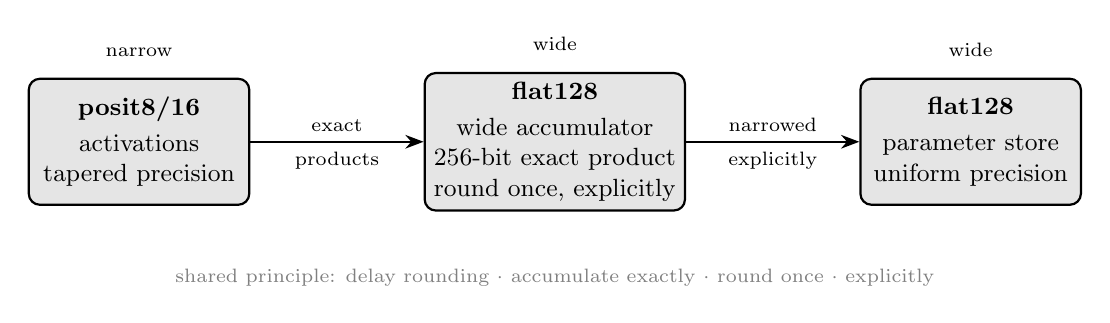
\begin{tikzpicture}[
  node distance=1.6cm,
  box/.style={rectangle,rounded corners=4pt,draw,thick,
              minimum width=2.8cm,minimum height=1.6cm,
              align=center,fill=black!10},
  arrow/.style={-{Stealth},thick},
  font=\small
]
  \node[box] (posit) {\textbf{posit8/16}\\[2pt]activations\\tapered precision};
  \node[box,right=2.2cm of posit] (flat) {\textbf{flat128}\\[2pt]wide accumulator\\256-bit exact product\\round once, explicitly};
  \node[box,right=2.2cm of flat]  (store) {\textbf{flat128}\\[2pt]parameter store\\uniform precision};
  \node[font=\scriptsize,above=0.15cm of posit] {narrow};
  \node[font=\scriptsize,above=0.15cm of flat]  {wide};
  \node[font=\scriptsize,above=0.15cm of store] {wide};
  \draw[arrow] (posit) -- node[above,font=\scriptsize]{exact}
                           node[below,font=\scriptsize]{products} (flat);
  \draw[arrow] (flat)  -- node[above,font=\scriptsize]{narrowed}
                           node[below,font=\scriptsize]{explicitly} (store);
  \node[font=\scriptsize,gray,below=0.6cm of flat]
        {shared principle: delay rounding $\cdot$ accumulate exactly
         $\cdot$ round once $\cdot$ explicitly};
\end{tikzpicture}
\caption{Proposed pipeline division of labor. Posit8/16 concentrates
precision where activation distributions are dense. Flat128 accumulates
exact 256-bit intermediate products at the wide stage. Parameters are
stored at uniform flat128 precision. All three stages share one
principle: round once, explicitly, at a defined boundary, and never
invisibly inside an operation.}
\label{fig:pipeline}
\end{figure}
\subsection{Encoding vs. Accumulation}
Our synthesis frame: posits solves the \emph{encoding} problem (where do
bits go within a word); flat128 solves the \emph{accumulation} problem
(where do bits go across operations). Both attack the same root cause.
The ISA should support both without forcing a choice.

Neither format removes the hard parts: softmax, sigmoid, normalization,
outliers, dynamic rescaling, and transcendental approximation each
require independent treatment. The principle both share --- delay
rounding, accumulate exactly, round once explicitly --- is the
non-negotiable kernel. The encoding question remains open.


Figure~\ref{fig:partial} illustrates the partial-product structure
underlying \texttt{Mult128.c}~\cite{sherman2026mult128}. Each 128-bit
operand is partitioned into four 32-bit limbs; the full $128\times128$
product decomposes into sixteen $32\times32$ partial products, each
computable by a single \texttt{MUL} instruction in base RV64I\@.
No exotic hardware is required, this is the same long multiplication
learned in primary school, scaled to 128-bit limbs.

\begin{figure}[h]
\centering
\resizebox{\linewidth}{!}{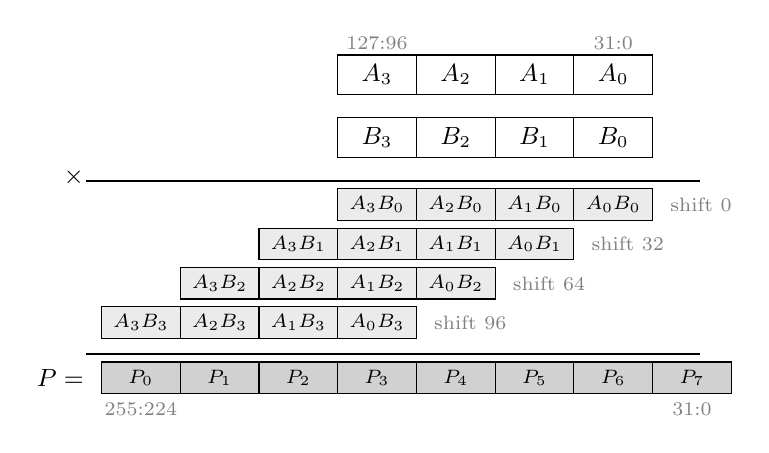
\begin{tikzpicture}[font=\small]
  % Operand A — right-aligned
  \foreach \i/\l in {3/$A_3$,4/$A_2$,5/$A_1$,6/$A_0$} {
      \draw (\i,2) rectangle (\i+1,2.5);
      \node at (\i+0.5,2.25) {\l};
  }
  \node[font=\scriptsize,gray] at (3.5,2.65) {127:96};
  \node[font=\scriptsize,gray] at (6.5,2.65) {31:0};
  % Operand B — right-aligned
  \foreach \i/\l in {3/$B_3$,4/$B_2$,5/$B_1$,6/$B_0$} {
      \draw (\i,1.2) rectangle (\i+1,1.7);
      \node at (\i+0.5,1.45) {\l};
  }
  % multiply sign and rule
  \node[anchor=east] at (-0.1,0.95) {$\times$};
  \draw[thick] (-0.2,0.9) -- (7.6,0.9);
  % Row 0: A x B0, shift 0 — rightmost position
  \foreach \i/\l in {3/$A_3 B_0$,4/$A_2 B_0$,5/$A_1 B_0$,6/$A_0 B_0$} {
      \draw[fill=black!8] (\i,0.4) rectangle (\i+1,0.8);
      \node[font=\scriptsize] at (\i+0.5,0.6) {\l};
  }
  \node[font=\scriptsize,gray,anchor=west] at (7.1,0.6) {shift 0};

  % Row 1: A x B1, shift 32
  \foreach \i/\l in {2/$A_3 B_1$,3/$A_2 B_1$,4/$A_1 B_1$,5/$A_0 B_1$} {
      \draw[fill=black!8] (\i,-0.1) rectangle (\i+1,0.3);
      \node[font=\scriptsize] at (\i+0.5,0.1) {\l};
  }
  \node[font=\scriptsize,gray,anchor=west] at (6.1,0.1) {shift 32};
  % Row 2: A x B2, shift 64
  \foreach \i/\l in {1/$A_3 B_2$,2/$A_2 B_2$,3/$A_1 B_2$,4/$A_0 B_2$} {
      \draw[fill=black!8] (\i,-0.6) rectangle (\i+1,-0.2);
      \node[font=\scriptsize] at (\i+0.5,-0.4) {\l};
  }
  \node[font=\scriptsize,gray,anchor=west] at (5.1,-0.4) {shift 64};
  % Row 3: A x B3, shift 96 — leftmost position
  \foreach \i/\l in {0/$A_3 B_3$,1/$A_2 B_3$,2/$A_1 B_3$,3/$A_0 B_3$} {
      \draw[fill=black!8] (\i,-1.1) rectangle (\i+1,-0.7);
      \node[font=\scriptsize] at (\i+0.5,-0.9) {\l};
  }
  \node[font=\scriptsize,gray,anchor=west] at (4.1,-0.9) {shift 96};
  % sum rule and result
  \draw[thick] (-0.2,-1.3) -- (7.6,-1.3);
  \node[anchor=east] at (-0.1,-1.6) {$P=$};
  \foreach \i in {0,...,7} {
    \draw[fill=black!18] (\i,-1.8) rectangle (\i+1,-1.4);
    \node[font=\scriptsize] at (\i+0.5,-1.6) {$P_\i$};
  }
  \node[font=\scriptsize,gray] at (0.5,-2.0) {255:224};
  \node[font=\scriptsize,gray] at (7.5,-2.0) {31:0};
\end{tikzpicture}}
\caption{$128\times128$-bit multiplication as sixteen $32\times32$
partial products --- long multiplication scaled to 128-bit limbs.
Each $A_i B_j$ term maps to one \texttt{MUL} in base RV64I\@;
rows shift left by 32 bits per $B$ limb index.
The 256-bit result $P_0$--$P_7$ is exact with no intermediate rounding.}
\label{fig:partial}
\end{figure}


% ---- METHODS ----
\section{Methods}\label{sec:methods}
\subsection{Division of Labor: Experimental Hypothesis}

The following is proposed as a research hypothesis, not an architectural
conclusion. Measured accuracy, latency, energy, and overflow incidence
results against FP8, BF16, integer quantization, and existing RVV
widening paths are required before any column below hardens into a
recommendation.

\begin{table}[h]
\centering
\caption{Proposed division of labor by pipeline stage (hypothesis only).}
\label{tab:division}
\begin{tabularx}{\textwidth}{l@{\hspace{1.5em}}p{1.6cm}@{\hspace{1.5em}}L}
\toprule
\textbf{Format} & \textbf{Width} & \textbf{Proposed use and what needs measuring} \\
\midrule
Posit8/16 & Narrow & Activations where tapered precision matches
  weight/activation distributions.
  Accuracy vs.\ FP8/BF16; calibration cost; outlier behavior. \\
Float32/BFloat16 & Medium & Current training baseline:
  comparison target.
  Already measured; literature available. \\
Flat128 & Wide & Auditable high-precision reference reductions;
  deterministic scientific kernels; selected training accumulators.
  Overflow incidence; scale-management overhead;
  cycles and energy vs.\ FMA/RVV. \\
\bottomrule
\end{tabularx}
\end{table}

A more defensible near-term target than general NN inference is:
auditable high-precision reference reductions, deterministic scientific
kernels, compensated and reproducible reductions, and selected training
accumulators where exact intermediate results are architecturally
required.

\subsection{Reproducibility Argument}

IEEE~754 permits rounding-mode variation across implementations, making
training reproducibility across hardware vendors a persistent practical
burden. Flat128 can make a specified fixed-point reduction bitwise
reproducible across conforming implementations, without per-operation
rounding, provided the specification fixes:
\begin{enumerate}
\item input encoding and scale,
\item product width and reduction order,
\item overflow behavior, and
\item narrowing rule and distributed-reduction protocol.
\end{enumerate}

This is meaningful and measurable. Our claim is narrower and stronger
than a general reproducibility guarantee: flat128 accumulation eliminates
the per-operation rounding decision entirely, making the reproducibility
contract simpler to specify, verify, and audit. For distributed training,
reproducibility additionally requires fixed shard ordering, collective
topology, deterministic kernels, and defined overflow handling. Flat128
simplifies that stack; it does not by itself guarantee it.
Iterative refinement with posit arithmetic offers a complementary
approach at the narrow operand layer~\cite{quinlan2024iterative}.

\subsection{Experimental Setup}

Experiments are conducted on the Milk-V Pioneer SG2042, a 64-hart
RISC-V server (Debian sid, GCC 13.3.0, 128\,GB DDR4, four NUMA nodes),
using the Universal Numbers Library~\cite{omtzigt2023universal} for
arithmetic type validation.
This represents the first known empirical evaluation of flat128
accumulation on production RISC-V silicon. Dot products of $K \in
\{64, 128, 256, 512, 1024, 2048, 4096\}$ elements are accumulated under
flat128 fixed-point and IEEE~754 double-precision using 1 and 64
concurrent threads, spanning all four NUMA nodes.

\subsection{ISA Encoding Sketch}

\begin{itemize}
\item 32-bit instruction word preserved.
\item New major opcode block for \texttt{q128} operations.
\item \texttt{funct3} distinguishes: \texttt{LDQW}, \texttt{STQW},
  \texttt{MACQW}, \texttt{CVTQW}.
\item Three register fields (rs1, rs2, rd) at 5 bits each + opcode +
  funct3 = 32 bits exact.
\item No R5 needed; no encoding gymnastics. Same six instruction forms:
  R(4), I, S, B, U, J.
\end{itemize}

Note: this is an encoding sketch. Register file definition, calling
convention, context-switch state, and ABI remain open architectural
questions for the full proposal, targeted as a complete RFC submission
to RISC-V International by Q4~2026.\footnote{Implementation and reproducibility results: \url{https://github.com/psherman42/flat128}}

\subsection{Register File Architecture}

\begin{table}[h]
\centering
\caption{Register file alternatives for flat128.}
\label{tab:regfile}
\begin{tabularx}{\textwidth}{lLLL}
\toprule
\textbf{Alternative} & \textbf{Description} & \textbf{Pros} & \textbf{Cons} \\
\midrule
RV128 x-registers & Use existing 128-bit GP registers & Zero new register file; lowest ISA surface & Competes with pointers; gates on RV128 adoption \\
RV64 register pairs & Two adjacent 64-bit x-registers per operand & Leverages \texttt{\_\_int128}; works today & High register pressure; awkward pair allocation \\
RVV widening accumulation & Vector extension widening/accumulation & Best throughput for inference kernels & Scalar 128-bit not the target; accumulator lifecycle needs definition \\
Dedicated accumulator & New wider architectural accumulator register(s) & Strong for exact dot products & Save/restore; interrupt/trap behavior; maximum dot length must be defined \\
\bottomrule
\end{tabularx}
\end{table}

Note: a separate q128 register file, implied by the current ISA
encoding sketch, is not a low-friction addition. It creates register
allocation and spilling work, context-switch and virtualization state,
debugger and unwinder support, assembler and disassembler work, and a
new ABI class. The recommended path: prototype on RV64 register pairs
using existing \texttt{\_\_int128} before proposing a new register file.
Demonstrate LLVM IR representation and lowering first.

\subsection{Binary Point and Arithmetic Contract}

\begin{table}[h]
\centering
\caption{Open binary point and arithmetic contract questions.}
\label{tab:binarypoint}
\begin{tabularx}{\textwidth}{p{1.8cm}@{\hspace{1.5em}}>{\raggedright\arraybackslash}p{0.42\textwidth}@{\hspace{1.5em}}L}
\toprule
\textbf{Question} & \textbf{Options} & \textbf{Current position} \\
\midrule
Scale & Fixed globally; per-type; per-instruction; compiler metadata & Compiler-tracked \\
Addition & Unlike scales: illegal; implicit shift; explicit convert & Position required \\
Multiplication & Return 256-bit pair; scaled 128-bit with rounding; both & Full 256-bit pair \\
Overflow & Modular wrap; saturating; trap; sticky overflow flag & Position required \\
Rounding & Truncate; round-to-nearest-even; stochastic; explicit shift & Truncate \\
Conversion & FP$\leftrightarrow$flat128: overflow, NaN/Inf handling, exact semantics & Position required \\
Memory ABI & Alignment, endianness, atomics, DWARF, calling convention & Position required \\
\bottomrule
\end{tabularx}
\end{table}

\FloatBarrier

% ---- RESULTS ----
\section{Results}\label{sec:results}
\subsection{Flat128 Reproducibility}

Table~\ref{tab:results} reports dot product accumulation results on the
SG2042 Pioneer (64-hart RISC-V, four NUMA nodes, Debian sid, GCC~13.3.0)
across thread counts $T \in \{1, 4, 16, 64\}$ and vector lengths
$K \in \{64, 128, 256, 512, 1024, 2048, 4096\}$.

Flat128 produces bitwise-identical results across all $K$ and $T$.
IEEE~754 double-precision diverges first at $K=128$ (relative error
$8.7\times10^{-16}$), reaching $8.9\times10^{-16}$ at $K=4096$.
Divergence shows no monotonic trend with $K$, consistent with
nondeterministic thread scheduling rather than accumulated rounding error.

\begin{table}[h]
\centering
\caption{Flat128 vs.\ IEEE~754 double-precision dot product accumulation
on SG2042 Pioneer. Flat128 hex result (most significant limb) is
bitwise identical across all runs; double relative error is
$(\max - \min)/\min$ across thread counts $T \in \{1,4,16,64\}$.}
\label{tab:results}
\begin{tabular}{r@{\hspace{1em}}c@{\hspace{1em}}c@{\hspace{1em}}r}
\toprule
$K$ & Flat128 (hex, limb[3]) & Identical & Double rel.\ error \\
\midrule
64   & \texttt{002b4c60} & $\checkmark$ & $0$ \\
128  & \texttt{014d08c0} & $\checkmark$ & $8.7\times10^{-16}$ \\
256  & \texttt{0a33d180} & $\checkmark$ & $8.8\times10^{-16}$ \\
512  & \texttt{50cea300} & $\checkmark$ & $4.4\times10^{-16}$ \\
1024 & \texttt{83394600} & $\checkmark$ & $1.1\times10^{-15}$ \\
2048 & \texttt{0ce28c00} & $\checkmark$ & $8.9\times10^{-16}$ \\
4096 & \texttt{33851800} & $\checkmark$ & $8.9\times10^{-16}$ \\
\bottomrule
\end{tabular}
\end{table}

\begin{figure}[h]
\centering
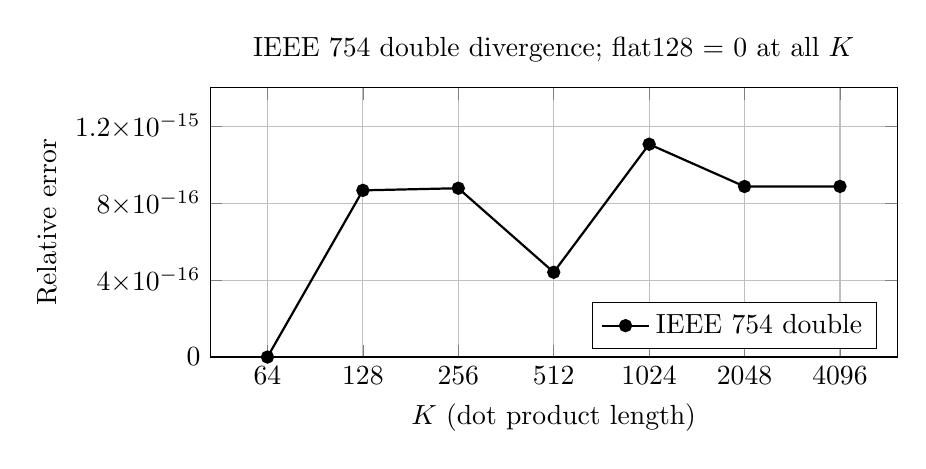
\begin{tikzpicture}
\begin{axis}[
    width=0.85\textwidth,
    height=5cm,
    xlabel={$K$ (dot product length)},
    ylabel={Relative error},
    xmode=log,
    log basis x=2,
    xtick={64,128,256,512,1024,2048,4096},
    xticklabels={64,128,256,512,1024,2048,4096},
    ymin=0, ymax=1.4e-15,
    ytick={0,4e-16,8e-16,1.2e-15},
    % yticklabel style={/pgf/number format/sci}, % misbehaving, use two lines below
    scaled y ticks=false,
    yticklabels={0,$4{\times}10^{-16}$,$8{\times}10^{-16}$,$1.2{\times}10^{-15}$},
    grid=major,
    legend pos=south east,
    title={IEEE~754 double divergence; flat128 = 0 at all $K$},
]
\addplot[color=black, mark=*, thick] coordinates {
    (64,   0)
    (128,  8.67e-16)
    (256,  8.78e-16)
    (512,  4.41e-16)
    (1024, 1.107e-15)
    (2048, 8.87e-16)
    (4096, 8.875e-16)
};
\addlegendentry{IEEE 754 double}
\end{axis}
\end{tikzpicture}
\caption{Relative divergence $(\max-\min)/\min$ of IEEE~754 double-precision
dot product across $T \in \{1,4,16,64\}$ threads on SG2042 Pioneer.
Flat128 divergence is identically zero at all $K$.}
\label{fig:divergence}
\end{figure}

\subsection{NUMA Locality}

To isolate the effect of NUMA topology, threads were pinned to individual
NUMA nodes using \texttt{numactl --cpunodebind}. Under single-node
pinning at $K=4096$, $T=16$, both flat128 and IEEE~754 double produce
identical results across all four nodes (Table~\ref{tab:numa}),
confirming that double's divergence in the unpinned case arises from
nondeterministic cross-NUMA thread scheduling rather than from arithmetic
non-associativity alone. Flat128 produces bitwise-identical results
regardless of pinning, immune to scheduling order by construction.

\begin{table}[h]
\centering
\caption{NUMA locality test: $K=4096$, $T=16$, pinned per node.
Flat128 hex and double result are identical across all four NUMA nodes.}
\label{tab:numa}
\begin{tabular}{c@{\hspace{1.5em}}c@{\hspace{1.5em}}c}
\toprule
NUMA node & Flat128 (limb[3:2]) & Double result \\
\midrule
0 & \texttt{000000a0 33851800} & $5.0745\times10^{30}$ \\
1 & \texttt{000000a0 33851800} & $5.0745\times10^{30}$ \\
2 & \texttt{000000a0 33851800} & $5.0745\times10^{30}$ \\
3 & \texttt{000000a0 33851800} & $5.0745\times10^{30}$ \\
\bottomrule
\end{tabular}
\end{table}

\subsection{Performance}

$K=4096$ with $T=64$ threads completes in 23\,ms wall time on the SG2042
Pioneer (\texttt{time ./flatdot 4096 64}), including thread spawn and
join overhead. This is a software emulation of flat128 arithmetic in
portable C with no custom RISC-V ISA extensions. A hardware
implementation mapping each 128-bit addition to four 32-bit RV64I
operations would reduce this further.


% ---- CONCLUSIONS ----
\section{Conclusions}\label{sec:conclusions}
\subsection{The Deployment Axis}
\looseness=-1

It is not precision versus usefulness as opposites. Rather, it is
precision versus deployability friction. A perfect arithmetic that nobody
ships is a math paper. A deployable and maintainer-friendly arithmetic
with known precision limits that ships in 10,000 nodes wins. We know
this from the storage industry and from RISC-V adoption history.

Posit precision is excellent: tapered where it counts, the quire architecturally beautiful. Yet posits' deployment friction is real: toolchain support is nearly zero outside research groups; there is no IEEE~754 compatibility layer; every existing numerical library breaks; the compiler does not know what a posit is; hardware requires custom decode with no FPU reuse. The elegance of posits has not translated to adoption in over ten years. This is worth naming honestly, not as a criticism of Gustafson, but as the deployment gap this work is trying to close.

Flat128 precision is uniform and exact for addition, explicit for multiply, and arguably less elegant than posit: no taper, no quire magic. Its deployment friction is surprisingly low, however: two's complement integer arithmetic is understood by every compiler; GCC and LLVM \texttt{\_\_int128} exist today; no new number format is needed in the toolchain; a maintainer reading the patch sees new opcodes, wider registers, and integer semantics, nothing architecturally alien; and IEEE~754 libraries continue to work alongside it.

\subsection{The Maintainer-Friendly Argument}

A skeptical kernel maintainer reading an RFC for flat128 should find:
\begin{itemize}
  \setlength{\itemsep}{4pt}
  \item No new number format in the compiler --- \texttt{\_\_int128}
  already exists; extend it.
  \item ABI impact depends on register file choice (see
  Section~\ref{sec:methods}).
  \item Optional extension --- implementations that do not want hardware
  support can trap and emulate.
  \item No new rounding modes --- truncation is explicit in the
  instruction.
  \item Fallback story: if we have float128, we have 90\% of this already;
  flat128 removes the 15 exponent bits of overhead.
\end{itemize}

Float128 already exists in the RISC-V specification. Flat128 is
conceptually float128 minus the exponent field. Framed that way, it is
less radical than what has already been ratified.

\subsection{Open Questions}

\begin{itemize}
  \setlength{\itemsep}{4pt}
  \item What is our position on accumulator width --- is the quire separate
  from register space, or are we open to register-width accumulation?
  \item Overflow semantics: two's complement wrap, saturating, trap, or
  sticky overflow?
  \item Multiply result: full 256-bit pair, truncated 128, or implicit MAC
  accumulation into wider state?
  \item Quire as separate architectural state vs.\ flat128 register ---
  needs a position.
  \item Hardware cost: 128-bit adder is cheap; $128\times128$ multiply
  equals four $64\times64$ MUL/MULHU pairs already available in base
  RV64I; hardware single-cycle extension is incremental.
  \item Related work sweep: IBM hexadecimal float, DEC VAX G-float,
  various fixed-point DSP ISAs --- distinguish clearly.
\end{itemize}

\subsection{The Place of Contention}

Some prefer posits as the format at every width including wide, with
the quire as the accumulator mechanism: a unified posit world where fixing the
encoding causes everything else to follow. Others prefer integer semantics
for the wide accumulator, with posits narrow and flat128 wide
coexisting: deployability first, elegance where it is free.

This paper does not resolve that tension artificially. Both positions
share one architectural principle: exact intermediate results. The
encoding question is open. Advancing the principle is the contribution.


% ---- Bibliography ----
 \bibliographystyle{splncs04}
 \bibliography{references}
%

%\newpage 
% \appendix
% \section{Results Tables for MatrixDepot}\label{app:c}
% \input{sections/appc}
% \FloatBarrier
% \newpage 
% \section{Experiment 1 Code}
% \input{sections/x1}
% \newpage
% \section{Experiment 2 Code}
% \input{sections/x2}

\end{document}
